\chapter[Proposta de Trabalho]{Proposta de Trabalho}

A proposta de trabalho consiste no desenvolvimento de uma aplicação descentralizada(Dapp), por meio do Ethereum, para o registro de infrações de trânsito utilizando-se da tecnologia \textit{blockchain} para garantir a integridade das informações registradas. 

Será implementado um blockchain do tipo público, onde todos podem contribuir para o processo de consenso e validação dos blocos adicionados, possibilitando que qualquer pessoa interessada possa contribuir para a rede de registros se tornando um nó para validar as transações. Para mais informações em relação a este tipo de blockchain, veja a Seção \ref{subsection_tipos_blockchain}

Para auxiliar nos testes e uso da aplicação descentralizada durante o desenvolvimento, serão utilizadas duas ferramentas: Ganache e o Metamask. 

O Ganache \footnote{https://www.trufflesuite.com/docs/ganache/quickstart} permite ativar e gerenciar rapidamente um blockchain Ethereum pessoal para executar testes, executar comandos e inspecionar o estado do mesmo enquanto controla como a cadeia de blocos opera tanto pelo terminal de operações do computador como por uma interface gráfica. Dessa maneira pode-se testar os contratos inteligentes desenvolvidos sem o custo da rede Ethereum principal. 

O Metamask \footnote{https://metamask.io/} é uma carteira virtual e pode ser adicionada ao navegador como um plugin, que serve como uma ponte para conectar-se à rede desejada e injetar uma instância web3 no código. O Metamask possibilita selecionar e navegar entre diferentes redes (como uma rede local ou a principal Ethereum), assim como disponibiliza uma interface para gerenciar uma carteira digital com diferentes contas. Esta funcionalidade possibilitará que os diferentes níveis de restrições de usuários, como o usuário normal e o administrador, sejam testados durante todo o processo de desenvolvimento de forma prática.




Para a realização do trabalho, algumas premissas serão tomadas como base para seu desenvolvimento. As premissas são:

    \begin{enumerate}
        \item O sistema funcionará como o RENAINF(vide Seção \ref{section_renainf}), ou seja o sistema único para registro de infrações em todo o território nacional, onde todas infrações serão registradas nesta plataforma, mesmo caso o infrator tenha o carro licenciado na unidade federativa onde ocorreu a violação da norma;
        \item Cada órgão ou entidade do sistema nacional de trânsito terá sua representação no sistema por meio de uma conta de administrador;
        \item Serão utilizados bancos de dados auxiliares para simular as bases de dados de condutores habilitados e veículos registrados, de forma que essas informações possam ser obtidas para o registro da infração;
        \item Cada condutor habilitado terá seu próprio conjunto de chaves público/privada, onde a chave pública será salva junto ao registro do condutor no banco de dados auxiliar responsável por esta informação.
    \end{enumerate}


\section{Aplicação proposta}

Uma aplicação descentralizada será criada para tornar o processo de registro infrações de trânsito transparente e descentralizado. A biblioteca React escrita em javascript será usado para implementar o \textit{front-end} e os contratos inteligentes da plataforma Ethereum serão usados no \textit{back-end}. 

O ReactJs é uma biblioteca javaScript usada para criar interfaces de usuário. A principal característica é que podemos criar nossos aplicativos de maneira modular, o que ajuda a reduzir a repetição de códigos e facilita a depuração. Ele também permite modificar os elementos HTML dinamicamente, facilitando a criação de páginas interativas em tempo real. 

Os contratos inteligentes escritos em \verb|solidity| para a rede Ethereum no back-end da aplicação torna o Dapp descentralizado e transparente. A linguagem \verb|solidity| também é totalmente suportada pelo Ethereum e tem uma grande comunidade ao seu redor, o que auxilia no aprendizado e na solução de possíveis empecilhos ao longo do desenvolvimento do projeto.

\subsection{Arquitetura Proposta}

A arquitetura da aplicação será no estilo cliente servidor. O Dapp conterá duas partes principais: o contrato, sendo executado na rede Ethereum, e a aplicação cliente sendo executado localmente no computador do usuário.

Um exemplo dessa arquitetura pode ser vista na Figura \ref{fig:dapp_representacao}.

    \begin{figure}[h]
         \centering
         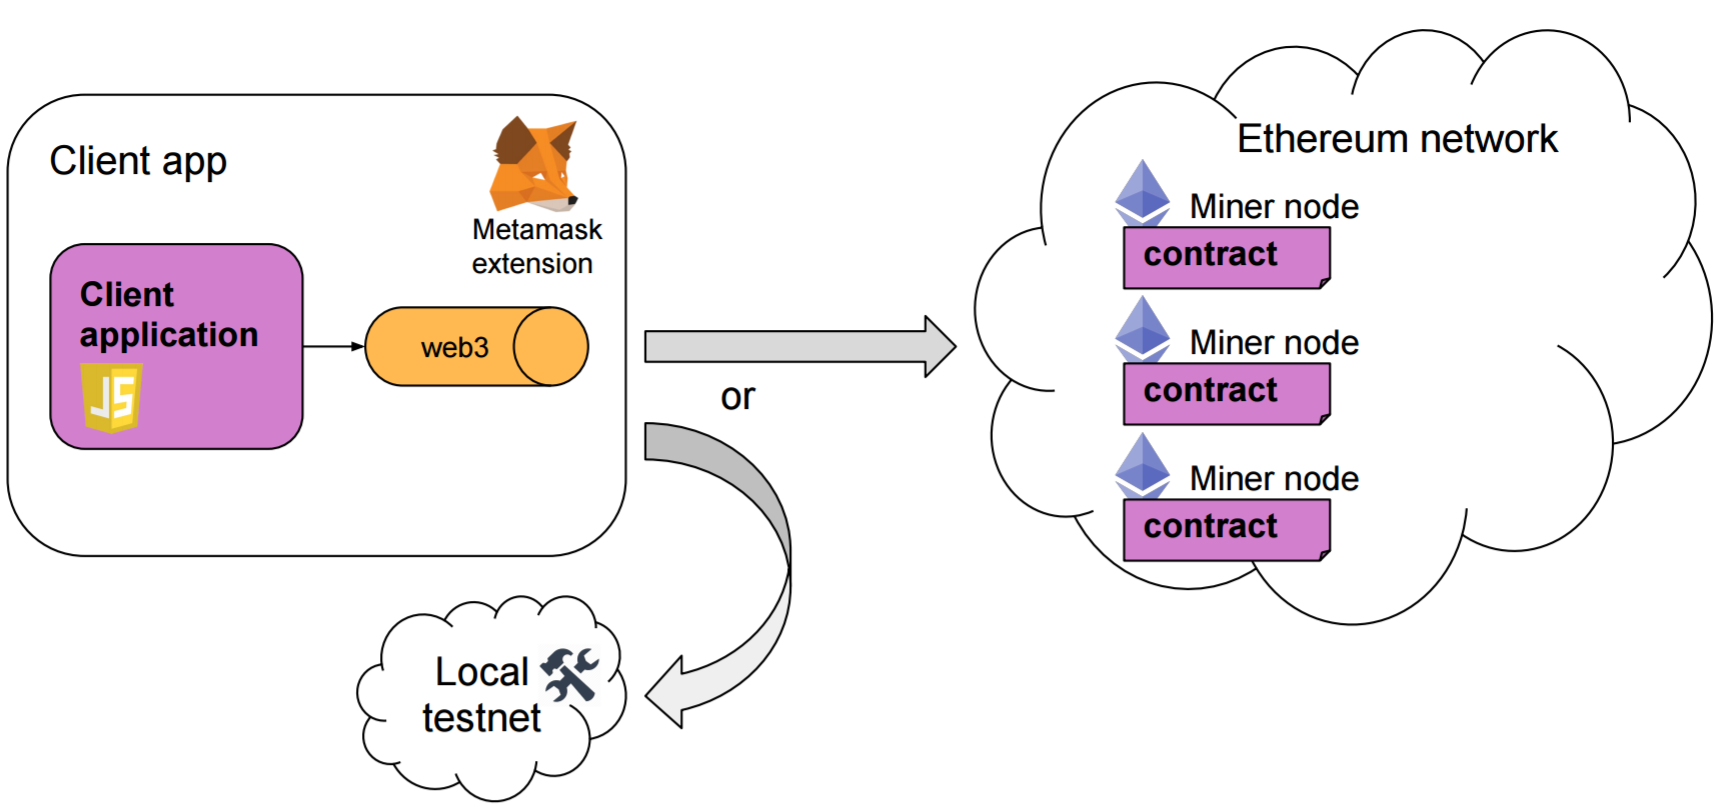
\includegraphics[scale=0.25]{figuras/capitulo_3/dapp_representacao_comunicacao.png}
         \caption{Representação das partes - Imagem retirada de \href{https://sites.google.com/site/blockchaintutorial/dapp-architecture}{Dapp Architecture}.}
         \label{fig:dapp_representacao}
    \end{figure}



\subsection{Funcionalidades}
\label{section:funcionalidades_propostas}

De forma a contemplar o máximo de situações contempladas no sistema RENAINF e respeitando a regulação presente no CTB, o sistema conterá as seguintes funcionalidades:


    \subsubsection{Registro de Infração}
    
        No registro de uma infração, os órgãos ou entidades registrados como administradores vão inserir no sistema as informações relacionadas ao registro de infração. Nesta plataforma inicialmente não serão registrados todos os campos elencados no CTB (Seção \ref{estrutura_auto_infracao}), as informações que serão cadastradas no sistema para o registro da infração de forma a contemplar as informações nesses campos são:
        
        \begin{quote}
        
            \begin{itemize}
                \item Placa do veículo
                \item Categoria da Infração
                \item Data/Hora da Infração
                \item Pontos da Infração
                \item Observações
                \item Chave do administrador responsável pelo registro
                \item Chave do motorista responsável pelo veículo
                \item Preço para pagamento da infração (valor em ethers)
            \end{itemize}
            
        \end{quote}
        
        Após confirmar as informações preenchidas, a transação será inserida no blockchain e validada por outros nós. Após este processo a infração estará disponível para que sejam realizadas as outras funções como consulta, realização de recursos e pagamento da mesma.
        
            
    \subsubsection{Transferência de Infração}
    
        Nesta funcionalidade, o usuário indicado como autor da infração registrada poderá transferir para outro usuário a autoria da infração de trânsito.
        
        Ao visualizar as informações da infração, o usuário(A) terá uma opção disponível para inserir a chave de outro usuário (B), e realizar a indicação de autoria. Este usuário (B) terá em sua página uma indicação dessa solicitação e terá disponível as opções: aceitar ou recusar. Caso o usuário (B) aceite a transferência assinando a transação com sua chave, a transação indicando a transferência será realizada de forma automática sem a necessidade da interferência de um usuário administrador (C).
    
    \subsubsection{Busca de Infrações}
    
        A busca de infrações consistirá em dois módulos diferentes: busca realizada pelo administrador e busca do usuário normal.
        
        O usuário registrado como administrador poderá consultar os registros de diferentes formas, como: infrações de um usuário específico, ou por um veículo.
        
        Já o usuário normal terá em sua página de acesso todas as infrações que foram registradas como ele sendo o autor da infração, não sendo possível visualizar as infrações realizadas por outros usuários.
    
    \subsubsection{Pagamento Infração}
    
        O pagamento da infração poderá ser realizada pelo usuário indicado como responsável pela infração. Para este pagamento serão utilizadas as moedas virtuais da rede Ethereum, de acordo com o valor indicado na infração acrescido das taxas necessárias para a realização da transação(GAS). O pagamento de uma infração corresponde à ação de transferir os valores referentes ao pagamento da infração para a conta da autoridade que registrou a infração.
    
    
    \subsubsection{Recurso / Cancelamento de uma infração}
    
        Ao visualizar a infração o usuário (A) indicado como responsável também poderá entrar com recurso em relação a infração registrada. Esta condição se aplica a casos onde o usuário não concorda com a infração registrada ou possui uma explicação plausível que pode acarretar na anulação da mesma.
        
        Para realizar esta ação o usuário (A) deverá clicar na opção disponível, preencher as informações solicitadas e assinar a solicitação usando sua chave. Essa solicitação irá para análise por parte de um usuário(B) administrador com perfil indicado como um Junta de Trânsito, e o mesmo poderá recusar ou aceitar a solicitação realizada.
        
        Caso o usuário (B) administrador aceite o recurso realizado, uma transação será inserida no blockchain anulando a infração registrada anteriormente e removendo a responsabilidade do usuário (A) em relação a mesma removendo as penalidades aplicadas anteriormente.
        
        
\subsection{Minerar moedas}

Para minerar moedas Ethereum é necessário ter um computador com alta capacidade de processamento. O papel destes mineradores é encontrar uma sequência que torne um bloco de transações compatível com o bloco anterior. Para isso, o computador precisa efetuar milhares de cálculos por segundo para encontrar a combinação perfeita, por isso que eles precisam ser extremamente potentes. Ao encontrar a sequência compatível, o minerador recebe uma recompensa para cada bloco que ele minerar. Essa recompensa foi criada com a intenção de pagar as pessoas que emprestam poder computacional para manter a rede funcionando.

De forma a incentivar a inserção do maior número de nós possíveis na rede atuando como mineradores, tornando a confiabilidade da rede ainda maior, o sistema englobará uma funcionalidade que permitirá que o pagamento das infrações registradas no blockchain seja feito utilizando essa recompensa monetária obtida por meio da mineração. Este incentivo beneficiará principalmente pessoas jurídicas que possuem uma grande frota de veículos automotores e serviços computacionais a disposição, como empresas locadoras de veículos e empresas de transporte urbano, pois estes poderão pagar as infrações realizadas por sua frota com um certo desconto em relação ao valor normal ao ajudar na manutenção da rede.
